% English manuscript draft. Compile from carlos/.
\PassOptionsToPackage{hypertexnames=false}{hyperref}
\documentclass[a4paper,fleqn,review]{cas-sc}

\usepackage[T1]{fontenc}
\renewcommand{\rmdefault}{lmr}
\renewcommand{\sfdefault}{lmss}
\renewcommand{\ttdefault}{lmtt}
\usepackage[numbers,sort&compress]{natbib}
\usepackage[english]{babel}
\usepackage{amsmath,amsfonts,amssymb}
\usepackage{graphicx}
\usepackage{booktabs}
\usepackage{makecell}
\usepackage{placeins}
\usepackage{float}
\usepackage{tikz}
\usetikzlibrary{positioning,arrows.meta}
\definecolor{figblue}{HTML}{1B416C}
\definecolor{figteal}{HTML}{087B76}
\definecolor{figink}{HTML}{1D2938}
\definecolor{figline}{HTML}{A4B1C0}
\definecolor{figgray}{HTML}{F3F6F9}
\usepackage{hyperref}
\RenewDocumentCommand{\printorcid}{}{}
\ExplSyntaxOn
\RenewDocumentEnvironment { keywords } { O{ Keywords } }
  {
    \tex_global:D \tex_setbox:D \g_stm_key_box = \vtop \bgroup
    \hsize=.25\textwidth
    \cs_new:Nn \sep: { \par }
    \cs_set_eq:NN \sep \sep:
    \parindent=0pt
    {\small A\,R\,T\,I\,C\,L\,E~I\,N\,F\,O } \par \skip_vertical:n { -3pt }
    \rule{.25\textwidth}{.2pt}\par\footnotesize
    \noindent \textit { #1 } \par
  }
  { \egroup }
\cs_set:Npn \__first_footerline:
  {
    \small\sffamily\__short_authors:\quad
    {\rmfamily\itshape Draft~for~author~review}
  }
\ExplSyntaxOff

\begin{document}
\let\WriteBookmarks\relax
\def\floatpagepagefraction{1}
\def\textpagefraction{.001}

\shorttitle{Top-$k$ texture descriptors: direct and margin-gated inference}
\shortauthors{C. Ayala and J. Delgado}
\title[mode=title]{Top-\texorpdfstring{$k$}{k} descriptor concatenation for texture classification: direct use versus margin-gated acquisition}
\tnotemark[1]
\tnotetext[1]{English manuscript draft for author review.}
\author[1]{Carlos Ayala}
\cormark[1]
\ead{carlos.ayala@est.fpuna.edu.py}
\credit{Conceptualization, Methodology, Software, Investigation, Formal analysis, Writing -- original draft}
\affiliation[1]{organization={Facultad Politécnica, Universidad Nacional de Asunción},
            addressline={Campus Universitario}, city={San Lorenzo}, state={Central}, country={Paraguay}}
\author[1]{Joaquín Delgado}
\ead{joaquin.delgado@est.fpuna.edu.py}
\credit{Conceptualization, Methodology, Software, Investigation, Formal analysis, Writing -- review and editing}
\cortext[1]{Corresponding author}

\begin{abstract}
Concatenating texture descriptors gives the classifier complementary information, but extracting every selected block for every image can be costly. We study two decisions on six texture datasets: how many blocks to retain and when to extract them. Four blocks, selected as an exploratory operating point, use about 15\% of the dimensionality of the 22-block concatenation. Relative to all 22 blocks, mean accuracy changes by $-0.31$ percentage points with a linear SVM and $+0.32$ with a residual multilayer perceptron (ResMLP). In 27 paired SVM conditions, a cascade that requests Top-4 when the initial score margin is small escalates 21.1\% of images on average. Its accuracy differs from direct Top-4 by $+0.01$ percentage points (95\% interval: $-0.17$ to $+0.19$), while projected extraction cost falls from 468.3 to 117.1 ms per image. The margin gate outperforms random escalation at the same number of requests in all 27 conditions. In a separate online panel, a margin-gated policy that escalates to an ensemble lowers mean latency in all twelve dataset--classifier combinations, with accuracy losses on KTH-TIPS2-b and higher 95th-percentile latency on Soil.
\end{abstract}

\begin{keywords}
texture classification \sep descriptor fusion \sep Top-$k$ \sep conditional inference \sep latency
\end{keywords}
\maketitle

\section{Introduction}

A histogram of local patterns, an oriented filter bank, and a pretrained network capture different aspects of a texture \citep{ojala2002lbp,haralick1979glcm,cimpoi2014dtd,cimpoi2016fisher}. Concatenation lets a single classifier use those signals jointly. The cost starts before classification: every extractor in the representation has to run on the new image. If one descriptor already supports a reliable decision for many inputs, the remaining extraction can be reserved for cases where the initial decision is uncertain.

We separate the choice of descriptor set from the decision to compute it. First, we add whole descriptor blocks in order of their individual validation scores and examine the trade-off between accuracy and vector size. We use four blocks as a compact operating point. We then hold the Top-4 classifier fixed and compare two policies on the same test images. The direct policy always constructs the vector; the cascade constructs it only when the two highest scores of an inexpensive first-stage classifier are close. Because both policies use the same Top-4 classifier, we can count which errors the gate sends to be corrected and which correct initial decisions are overwritten.

A matched-count randomized control isolates the effect of choosing \emph{which} images to escalate. That comparison uses paired cached predictions and an extraction cost model. We separately measure single-image latency for a related margin-gated ensemble and report how its mean latency, accuracy, and tail latency change across datasets.

\section{Related work}

Earlier work on texture recognition has selected an extractor subset for reuse across tasks \citep{puig2010selection} or combined color and texture descriptors before compressing the fused representation \citep{khan2015compact}. Our unit of selection is a whole descriptor block. Greedy forward selection measures a block's added value conditional on the existing subset. Individual ranking is cheaper to search, but it can overlook a block that is useful mainly in combination with others \citep{kohavi1997wrappers,guyon2003feature}.

Several texture classifiers illustrate different sources of complementarity. \citet{neshov2025aggregation} aggregate activations across layers of a single backbone, including BEiTv2. HyTexNet combines percentile-based local encoding with DenseNet-121 features \citep{gupta2026hytexnet}. \citet{chang2024cellnn} concatenate multiscale LBP and contours from deep cellular neural networks. DeepLumina augments deep color features with luminance information \citep{simon2022deeplumina}. Their published accuracies provide context under the evaluation protocols reported by the original authors.

Cascades and early exits allocate compute according to the input \citep{viola2001rapid,teerapittayanon2016branchynet,wang2018idk,han2021dynamic}. Cost-aware feature acquisition likewise decides whether to acquire further inputs \citep{xu2012greedy,nan2017adaptive,ma2019eddi}. Early exits decide how far to advance in a network; IDK cascades choose whether to send a query to another model. Selective classification characterizes the error of accepted predictions as a function of coverage \citep{geifman2017selective}. Our cascade predicts a class on every input. The margin determines whether to acquire the remaining blocks of a fixed concatenation. This leads to three outcomes of interest: accuracy on all images, the rate of escalation, and extraction cost.

\section{Method}

\subsection{From individual descriptors to a joint representation}

Let $z_j(x)\in\mathbb{R}^{d_j}$ denote descriptor $j$ for image $x$. We normalize each block separately so that its input scale does not dominate the concatenation. For an ordered set $S$ this gives
\begin{equation}
 v_S(x)=\mathop{\Vert}_{j\in S}\frac{z_j(x)}{\max(\lVert z_j(x)\rVert_2,10^{-12})},
 \qquad d_S=\sum_{j\in S}d_j.
\end{equation}
The head $h_S$ takes the resulting fixed-length vector and outputs one score per class. Figure~\ref{fig:pipeline} shows the difference between individual and joint inputs. The library has six classical descriptors and sixteen learned representations with frozen weights (Tables~\ref{tab:extractores-clasicos} and \ref{tab:extractores-aprendidos}).

\begin{figure}[pos=htbp]
\centering
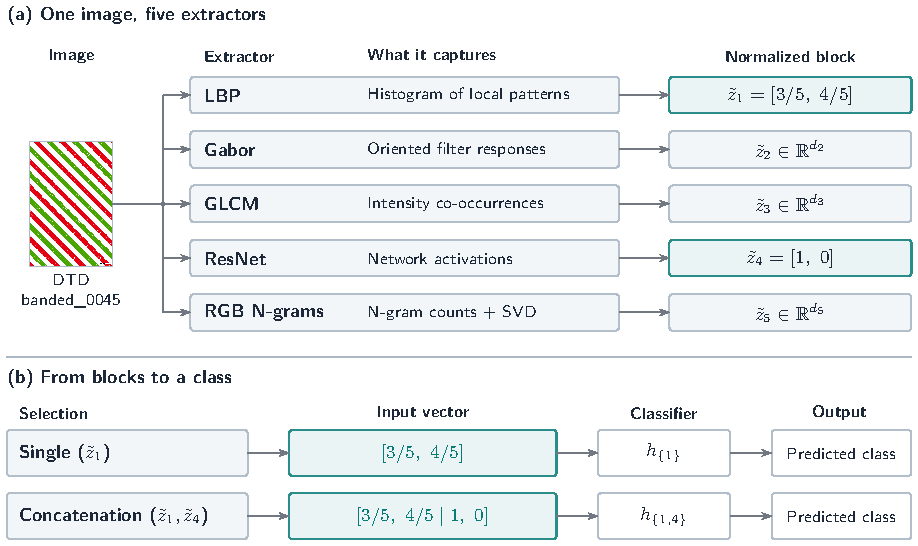
\includegraphics[width=\textwidth]{figures/english/descriptor_pipeline.pdf}
\caption{Extraction and concatenation for one image. Each extractor returns a normalized block. The individual head receives LBP. The joint head receives the concatenated LBP and ResNet blocks. The bar marks the block boundary; coordinates are illustrative.}
\label{fig:pipeline}
\end{figure}

Within each outer training split, we fit and score a head for each descriptor in the inner folds. We sort the descriptors by mean macro-F1, $\pi_1,\dots,\pi_{21}$, and take $S_k=(\pi_1,\ldots,\pi_k)$. RGB N-grams + SVD is reserved for the 22-block concatenation and a color ablation. Each condition has its own ranking. Direct Top-$k$ constructs $v_{S_k}$ for every image and predicts the highest-scoring class. Full-22 concatenates all 22 blocks. Single selects one block with the internal criterion of the static comparison.

\subsection{Margin-gated Top-$k$}

The first-stage head $h_b$ receives only descriptor block $b$. Let $s_{(1)}(x)$ and $s_{(2)}(x)$ denote its two highest scores. The output is
\begin{equation}
 m(x)=s_{(1)}(x)-s_{(2)}(x), \qquad
 \hat{y}(x)=
 \begin{cases}
 \operatorname*{arg\,max}_{c} h_{S_k}(x)_c, & m(x)\leq \tau_q,\\
 \operatorname*{arg\,max}_{c} h_b(x)_c, & m(x)>\tau_q.
 \end{cases}
 \label{eq:regla}
\end{equation}
Scores are one-versus-rest decision values for the SVM and logits for ResMLP. If the margin is small, the cascade extracts the missing blocks and returns the joint head's prediction. When $b\in S_k$, it reuses the first-stage block.

\begin{figure}[pos=htbp]
\centering
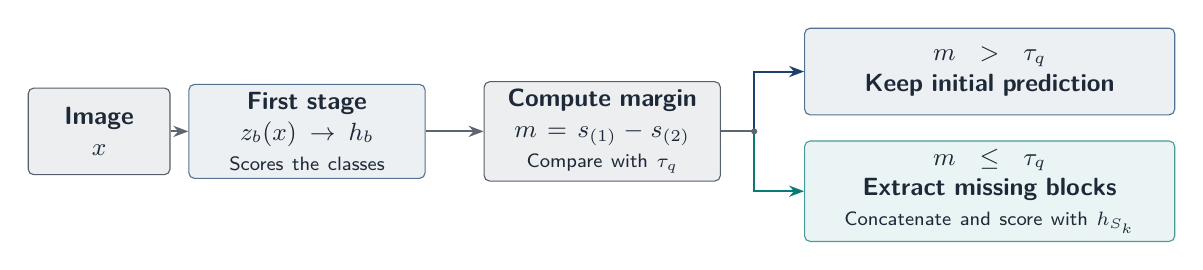
\begin{tikzpicture}[
  x=1cm, y=1cm, font=\sffamily\small, text=figink,
  caja/.style={rounded corners=2pt, draw=#1!75, fill=#1!8, align=center,
               text width=24mm, minimum height=11mm, inner sep=1mm},
  arr/.style={-{Stealth[length=1.9mm]}, line width=.72pt, draw=figink!72}
]
\node[caja=figink, text width=16mm] (img) at (.91,0) {\textbf{Image}\\$x$};
\node[caja=figblue, text width=28mm] (base) at (3.55,0)
  {\textbf{First stage}\\$z_b(x)\to h_b$\\ \scriptsize Scores the classes};
\node[caja=figink, text width=28mm] (gate) at (7.3,0)
  {\textbf{Compute margin}\\$m=s_{(1)}-s_{(2)}$\\ \scriptsize Compare with $\tau_q$};
\node[caja=figblue, text width=45mm] (out) at (12.22,.76)
  {$m>\tau_q$\\ \textbf{Keep initial prediction}};
\node[caja=figteal, text width=45mm] (top) at (12.22,-.76)
  {$m\leq\tau_q$\\ \textbf{Extract missing blocks}\\ \scriptsize Concatenate and score with $h_{S_k}$};
\draw[arr] (img) -- (base);
\draw[arr] (base) -- (gate);
\coordinate (split) at (9.23,0);
\draw[line width=.72pt,draw=figink!72] (gate.east) -- (split);
\draw[arr,draw=figblue] (split) |- (out.west);
\draw[arr,draw=figteal] (split) |- (top.west);
\fill[figink!72] (split) circle (1.1pt);
\end{tikzpicture}
\caption{Top-$k$ cascade. The margin is the gap between the two highest first-stage scores. Above $\tau_q$ the cascade retains the initial prediction. Otherwise it acquires any missing blocks and returns the joint prediction. The threshold is fixed before testing.}
\label{fig:cascada}
\end{figure}

The threshold $\tau_q$ is the $q$-quantile of the margins from out-of-fold predictions within the outer training split. The test escalation rate $\rho_q$ can differ from $q$. Let $C_j$ be the fixed extraction cost of block $j$ for the condition. The projected acquisition costs are
\begin{equation}
 C_{\mathrm{direct}}=\sum_{j\in S_k} C_j,\qquad
 C_{\mathrm{cascade}}= C_b + \rho_q \sum_{j\in S_k\setminus\{b\}}C_j.
 \label{eq:costos}
\end{equation}
Route selection uses the training escalation rate; reporting uses the observed test rate. If $b\in S_k$, the savings come from skipping the remaining blocks on a fraction $1-\rho_q$ of the inputs. Otherwise, savings require $(1-\rho_q)C_{\mathrm{direct}}>C_b$. The model sums extraction profiles and excludes classifier scoring and routing overhead.

For the Top-4 comparison we evaluated $q\in\{0.25,0.50,0.75\}$. Candidate first-stage blocks were ResNet-50, SigLIP-B, BEiTv2-B and ConvNeXt V2-T, with candidates restricted to ResNet-50 and BEiTv2-B for KTH-TIPS2-b. We chose the lowest projected-cost route whose out-of-fold macro-F1 was no more than 0.005 below direct Top-4. Direct use remained available if the candidates offered no admissible savings. The heads were refitted across the inner folds for threshold estimation, with the four blocks already fixed by the outer training split.

For each candidate block and quantile, we substitute the Top-4 prediction on inner out-of-fold calls at or below the candidate threshold. We compute macro-F1 on the pooled substituted predictions and compare it with the pooled macro-F1 of direct Top-4. Eligible routes compete on projected mean extraction cost. Exact cost ties favor direct Top-4 and then a ResNet-50 first stage among cascades. The selected heads are fitted on the full outer training split, and the selected threshold is applied unchanged. The quantile determines how the threshold is learned; the test margin distribution determines the test escalation rate.


\subsection{Margin-gated ensemble for online measurement}\label{sec:variante-panel}

The online policy chooses a first-stage block on the internal macro-F1 versus cost frontier and searches quantiles $\{0.10,0.25,0.50\}$. When $m(x)<\tau_q$, it aggregates the scores of up to three four-block concatenations from a diversity-based ensemble. The ensemble contains 15 subsets sampled using internal block relevance with a centered kernel alignment similarity penalty ($\lambda=0.25$, $\beta=8$) \citep{kornblith2019similarity}. The policy chooses the first stage, threshold, and escalation subsets to maximize three-fold internal macro-F1 under a projected mean budget of 60 ms. We refer to this policy as the \emph{margin-gated ensemble}; \emph{Top-4 cascade} refers to Equation~\eqref{eq:regla} with $k=4$.

\section{Experimental protocol}

A condition is defined by an outer split and an evaluation configuration. DTD uses its ten official tests, with the training and validation sets combined for inner selection and exact training duplicates of test images removed \citep{cimpoi2014dtd}. FMD and Soil use five stratified group folds for each of seeds 42, 123 and 2026 \citep{sharan2013fmd}. Soil comprises 1,140 original images after exact deduplication and groups related file families. CUReT uses two complementary halves of 46 capture conditions for 61 classes \citep{varma2003filter}. Outex uses an official TC 00013 split with 680 images on each side \citep{ojala2002outex}. KTH-TIPS2-b uses four splits that each hold out a complete physical sample per class \citep{mallikarjuna2005kth,scabini2023radam}.

The linear SVM uses $C=1$, balanced class weights, squared hinge loss, $L_2$ regularization, a tolerance of $10^{-4}$, and at most 10,000 iterations. ResMLP uses a width of 256, three residual blocks, layer normalization, GELU, and dropout of 0.1. AdamW uses a learning rate of $10^{-3}$, weight decay of $10^{-4}$, batch size 256, and at most 100 epochs. Early stopping restores the best training-loss checkpoint after ten epochs without an improvement of at least $10^{-4}$.

We use four stratified group folds within the outer training split for the sweep and the Top-4 cascade (Table~\ref{tab:protocolo}). Macro-F1 determines block rankings and route selection. Accuracy is the primary reported metric. Macro precision, recall and F1 treat classes equally and complement accuracy. E1 compares the policies with SVM using cached descriptors and extraction profiles. E4 refits the heads with ResMLP on the SVM-ranked blocks and reports accuracy. The online panel uses a single-image call on an RTX 4060 with resident extractors and prepared classifier heads.

\begin{table}[pos=htbp]
\centering
\caption{Main experiments. E1 and E4 share data splits and descriptor blocks.}
\label{tab:protocolo}
\small
\begin{tabular}{@{}p{.27\textwidth}p{.29\textwidth}p{.37\textwidth}@{}}
\toprule
Experiment & Coverage & Evidence \\
\midrule
Concatenation size & 47 conditions per head & Predictions from cached descriptors \\
\addlinespace
Direct Top-4 and Top-4 cascade & 27 conditions per head, seed 42 & Paired predictions and projected cost with SVM (E1). ResMLP uses the SVM-ranked blocks (E4) \\
\addlinespace
Margin-gated ensemble panel & 94 conditions, five policies & Accuracy and latency from the same single-image inference calls \\
\bottomrule
\end{tabular}
\end{table}

We average conditions within each dataset, then weight each dataset equally. Cross-dataset tests use the six datasets as paired units \citep{demsar2006statistical}. Outer splits may reuse images. The choice of $k=4$, the emphasis on accuracy, and the one-percentage-point noninferiority margin were made after observing results. The resulting comparisons are exploratory.

\subsection{Online timing boundary and aggregation}

For each test image, the harness runs the five frozen policies in randomized order. Two warm-up images per policy precede timed calls. The host starts a monotonic wall-clock timer after synchronizing the GPU and stops it after the policy predicts a class and the GPU synchronizes again. The timed interval begins with opening and decoding the image file. It includes RGB conversion, preprocessing, feature extraction and device-to-host transfer, block normalization, vector assembly, CPU scoring, and any routing or voting needed for the prediction. Loading weights, fitting heads, warm-up, and writing the timing records occur outside this interval. Table~\ref{tab:panel} reports the accuracy and elapsed time from the same calls.

The primary panel contains 94 split--classifier conditions, each with five policies and one measured repetition per image. Its 362,640 calls exclude the 9,400 calls in the additional DTD observation. The original DTD timing is retained. Hardware was shared, so timing reflects the conditions of these sessions. In particular, a recorded interruption affects the DTD mean. For the tail latency discussion, the 95th percentile is calculated over calls pooled within dataset, classifier and policy. Accuracy and mean latency in the main table average the split-level results within each dataset.

\section{Results}

\subsection{Accuracy and representation size}

SVM accuracy rises from 92.72\% with one block to 94.42\% with four. From five through 21 blocks it ranges from 94.33\% to 94.51\%. ResMLP reaches 94.20\% at four blocks and peaks at 94.43\% at five. Internal SVM macro-F1 peaks at six blocks (Figure~\ref{fig:curva-k}). Four blocks use roughly 3,150 of the 20,652 dimensions of Full-22. Rules that chose $k$ from the inner curves produced other sizes, so we treat four blocks as a practical operating point for studying the cascade.

\begin{figure}[pos=htbp]
\centering
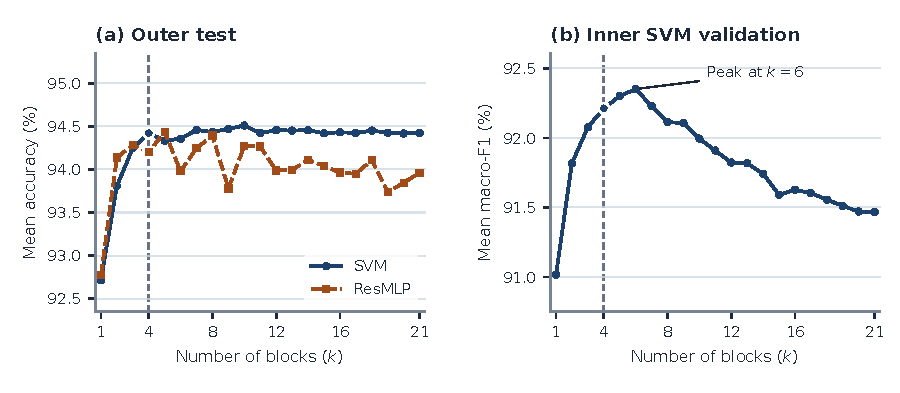
\includegraphics[width=\textwidth]{figures/english/curva_k.pdf}
\caption{Adding blocks in validation rank order. (a) Test accuracy with SVM and ResMLP. (b) Inner SVM macro-F1, which peaks at $k=6$. Each point averages within datasets and then across datasets. The vertical line marks $k=4$. The 21-block sweep excludes N-grams + SVD.}
\label{fig:curva-k}
\end{figure}

Top-4 improves on Single in eleven of twelve dataset--classifier comparisons, with mean accuracy 0.31 percentage points below Full-22 for SVM and 0.32 points above it for ResMLP (Table~\ref{tab:top4}). Outex accounts for the largest SVM decline (3.68 points). The exact Friedman tests across the three methods give $p=0.0521$ and $p=0.4297$ for SVM and ResMLP, respectively. No pairwise contrast reaches nominal significance after multiplicity adjustment. For the exploratory noninferiority comparison against Full-22, one-sided 95\% lower bounds are $-1.80$ points with SVM and $-0.64$ with ResMLP. Only the ResMLP bound exceeds the $-1$ point tolerance.

\begin{table}[pos=htbp]
\centering
\caption{Test accuracy of Single, Full-22 and Top-4, averaged over the outer conditions (47 per classifier). Outex has one official split. The last row gives mean representation dimension.}
\label{tab:top4}
\small
\begin{tabular}{@{}lrrrrrr@{}}
\toprule
 & \multicolumn{3}{c}{SVM} & \multicolumn{3}{c}{ResMLP} \\
\cmidrule(lr){2-4}\cmidrule(l){5-7}
Dataset & Single & Full-22 & Top-4 & Single & Full-22 & Top-4 \\
\midrule
DTD & 0.8448 & 0.8654 & \textbf{0.8703} & 0.8382 & \textbf{0.8635} & 0.8624 \\
FMD & 0.9727 & 0.9647 & \textbf{0.9823} & 0.9690 & 0.9563 & \textbf{0.9800} \\
CUReT & 0.9948 & \textbf{0.9989} & 0.9986 & 0.9971 & \textbf{0.9991} & 0.9984 \\
Outex & 0.9103 & \textbf{0.9662} & 0.9294 & \textbf{0.9485} & 0.9456 & 0.9368 \\
Soil & 0.9044 & \textbf{0.9281} & 0.9272 & 0.9044 & \textbf{0.9184} & 0.9149 \\
KTH-TIPS2-b & 0.9415 & \textbf{0.9609} & 0.9575 & 0.9099 & 0.9499 & \textbf{0.9596} \\
\midrule
Mean & 0.9281 & \textbf{0.9473} & 0.9442 & 0.9279 & 0.9388 & \textbf{0.9420} \\
Mean dimension & 873 & 20,652 & 3,144 & 656 & 20,652 & 3,170 \\
\bottomrule
\end{tabular}
\end{table}

Adding the RGB N-grams + SVD block raises mean SVM accuracy from 94.42\% to 94.89\%. Three datasets improve and three decline (Table~\ref{tab:e5-datasets}). Outex improves by 3.24 points, suggesting that a block outside the ranking can still complement the selected representation. SVD was fitted on training data for each condition. In the archived greedy forward selection comparison, Top-4 and forward selection obtain respectively 93.66\% and 92.95\% macro-F1 with SVM, and 93.31\% and 93.36\% with ResMLP.

\subsection{Which images benefit from escalation?}

Across 27 paired SVM conditions, mean accuracy is 94.44\% for direct Top-4 and 94.46\% for the cascade. The gate escalates 21.1\% of images on average and projected acquisition cost drops by 75.0\% (Table~\ref{tab:cascada}). Changes range from $-0.29$ percentage points on Outex to $+0.18$ on Soil (Figure~\ref{fig:e1-por-dataset}). With ResMLP on the SVM-ranked blocks, the gate escalates 22.5\% of images and obtains 94.24\% accuracy versus 94.28\% for direct use (Table~\ref{tab:e4-datasets}).

\begin{table}[pos=htbp]
\centering
\caption{Direct Top-4 and the Top-4 cascade with SVM on the same 27 test conditions (E1). $\Delta$ is cascade minus direct accuracy in percentage points before rounding. Extraction cost is projected from component profiles. The last row equally weights the datasets.}
\label{tab:cascada}
\small
\begin{tabular}{@{}lrrrrrrr@{}}
\toprule
 & & \multicolumn{3}{c}{Accuracy} & & \multicolumn{2}{c}{Projected cost (ms/image)} \\
\cmidrule(lr){3-5}\cmidrule(l){7-8}
Dataset & Cond. & Direct (\%) & Margin (\%) & $\Delta$ (pp) & Escalated (\%) & Direct & Margin \\
\midrule
DTD & 10 & 87.03 & 87.11 & $+0.09$ & 23.0 & 586.9 & 154.8 \\
FMD & 5 & 98.20 & 98.30 & $+0.10$ & 20.7 & 586.9 & 142.2 \\
CUReT & 2 & 99.86 & 99.79 & $-0.07$ & 20.0 & 625.6 & 148.2 \\
Outex & 1 & 92.94 & 92.65 & $-0.29$ & 19.9 & 608.7 & 141.9 \\
Soil & 5 & 92.89 & 93.07 & $+0.18$ & 23.6 & 130.0 & 50.7 \\
KTH-TIPS2-b & 4 & 95.75 & 95.83 & $+0.08$ & 19.3 & 271.7 & 64.5 \\
\midrule
Mean & 27 & 94.44 & 94.46 & $+0.01$ & 21.1 & 468.3 & 117.1 \\
\bottomrule
\end{tabular}
\end{table}
\begin{figure}[pos=htbp]
\centering
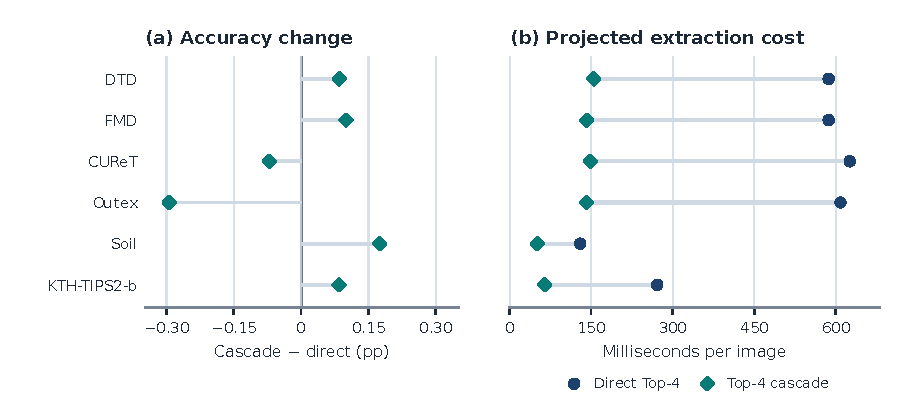
\includegraphics[width=\textwidth]{figures/english/comparacion_pareada_e1.pdf}
\caption{Accuracy and projected extraction cost for the Top-4 cascade by dataset (E1, 27 SVM conditions). (a) Cascade minus direct accuracy in percentage points. (b) Projected costs for the same conditions.}
\label{fig:e1-por-dataset}
\end{figure}

The first stage alone obtains 92.34\% mean SVM accuracy. Random escalation at the same count per condition gives 92.80\% over 100 draws per condition. Escalation by margin yields 94.46\% and outperforms this control in every condition. In the retrospective matched-count diagnostic (E2), the margin leads maximum score by 0.20 points and entropy by 0.47 points. The Holm-adjusted exact Wilcoxon $p$-values are 1.0000 and 0.8438 (Table~\ref{tab:e2-compuertas}). The adjusted tests leave the ordering of these uncertainty scores unresolved.

Of 31,984 predictions pooled across SVM conditions, 6,963 are escalated (21.8\%). They include 2,538 of the first stage's 3,483 errors. Always running Top-4 would correct 1,327 of those first-stage errors. The cascade captures 1,176 of the possible corrections (88.6\%) and turns 472 initially correct predictions into errors (Table~\ref{tab:e1-cambios}). It gains 135 correct predictions at the cost of one on CUReT. On DTD it gains 865 and loses 411.

Only calls that retain the first-stage prediction can change correctness relative to direct Top-4. On 168 such calls the first stage is correct and Top-4 is wrong; on 151, Top-4 would have corrected a first-stage error. No condition-level exact McNemar test reaches significance. The 95\% interval on the mean dataset-level accuracy difference is $[-0.17,+0.19]$ percentage points. In the exploratory noninferiority analysis, the one-sided $t$ bounds for both heads exceed $-1$ point (Table~\ref{tab:contrastes-margen}). The E1 two-sided Holm family compares the cascade with direct Top-4, a cascade restricted to ResNet-50, and Full-22. The noninferiority analysis was defined after observing E1.

\begin{table}[pos=htbp]
\centering
\caption{Changes in correctness (E1, 27 SVM conditions). An error is correctable when the first stage is wrong and Top-4 is correct. Corrected counts the subset selected by the gate. Lost and retained count correct first-stage predictions that Top-4 would get wrong, depending on whether the gate escalates. Totals may include images reused across splits.}
\label{tab:e1-cambios}
\small
\begin{tabular}{@{}lrrrrr@{}}
\toprule
 & & \multicolumn{2}{c}{First-stage errors} & \multicolumn{2}{c}{First-stage correct predictions} \\
\cmidrule(lr){3-4}\cmidrule(l){5-6}
Dataset & Escalated & Correctable & Corrected & Lost & Retained \\
\midrule
DTD & 4,316 & 1,006 & 865 & 411 & 157 \\
FMD & 207 & 17 & 17 & 4 & 1 \\
CUReT & 1,120 & 139 & 135 & 1 & 0 \\
Outex & 135 & 31 & 28 & 5 & 1 \\
Soil & 269 & 42 & 41 & 18 & 3 \\
KTH-TIPS2-b & 916 & 92 & 90 & 33 & 6 \\
\midrule
Total & 6,963 & 1,327 & 1,176 & 472 & 168 \\
\bottomrule
\end{tabular}
\end{table}
\begin{table}[pos=htbp]
\centering
\caption{Exploratory accuracy comparisons. Each test uses six paired dataset means. $\Delta$ is gated accuracy minus the comparator in percentage points. The noninferiority margin is one point.}
\label{tab:contrastes-margen}
\small
\setlength{\tabcolsep}{4pt}
\begin{tabular}{@{}p{.29\textwidth}rp{.24\textwidth}p{.315\textwidth}@{}}
\toprule
Comparison & $\Delta$ (pp) & Test & Result \\
\midrule
Margin vs.\ direct (E1, SVM) & $+0.01$ & Two-sided exact Wilcoxon & $p=0.5625$, $p_{\mathrm{Holm}}=1.0000$ \\
\addlinespace
Margin vs.\ random (E1, SVM) & $+1.66$ & Two-sided exact Wilcoxon & $p=0.0312$ unadjusted \\
\addlinespace
Margin vs.\ direct (E1, SVM) & $+0.01$ & Noninferiority & Lower bound 95\,\%: $-0.13$ pp \\
\addlinespace
Margin vs.\ direct (E4, ResMLP) & $-0.03$ & Noninferiority & Lower bound 95\,\%: $-0.21$ pp \\
\bottomrule
\end{tabular}
\end{table}


\paragraph{What the gate can change.}
For a paired test set of size $n$, let $A_i$ indicate a correct first-stage prediction, $T_i$ a correct direct Top-4 prediction, and $G_i$ an escalation. Cascade correctness on call $i$ is $A_i+G_i(T_i-A_i)$. Its accuracy differences from the first stage and direct Top-4 are
\begin{align}
 \Delta_{\mathrm{first}} &= n^{-1}\sum_{i=1}^{n}G_i(T_i-A_i),\\
 \Delta_{\mathrm{direct}} &= n^{-1}\sum_{i=1}^{n}(1-G_i)(A_i-T_i).
\end{align}
The first contrast counts corrections minus lost correct predictions among escalations. The second counts retained correct predictions minus missed corrections on the remaining calls. With the same Top-4 head in both policies, these identities give pooled gains of 704 correct predictions over the first stage and 17 over direct Top-4 in E1. The primary estimate weights datasets equally, so it describes a different aggregation from the pooled gain.

\subsection{Observed online latency}

The margin-gated ensemble lowers mean latency relative to direct Top-4 in all twelve dataset--classifier combinations. SVM latency falls from 245.06 to 39.93 ms per image, with accuracy changing from 94.23\% to 93.96\%. For ResMLP, latency falls from 232.76 to 36.10 ms and accuracy rises from 94.02\% to 94.39\%. On KTH-TIPS2-b, accuracy falls by 1.60 and 1.51 points respectively; on Outex it rises by 3.24 points with ResMLP. On Soil, even as mean latency drops, the 95th percentile rises from 117.6 to 136.7 ms for SVM and from 128.4 to 145.4 ms for ResMLP. Escalated inputs can incur the cost of both stages (Table~\ref{tab:panel}).

\begin{table}[pos=htbp]
\centering
\caption{Online panel of 94 conditions (\texttt{batch=1}, RTX 4060). Accuracy and latency (ms per image) use the same inference calls. The gate escalates to four-block subsets of a diversity-based ensemble.}
\label{tab:panel}
\small
\setlength{\tabcolsep}{4.5pt}
\begin{tabular}{@{}llrrrrrr@{}}
\toprule
 & & \multicolumn{2}{c}{Top-4} & \multicolumn{2}{c}{Margin ensemble} & \multicolumn{2}{c}{Full-22} \\
\cmidrule(lr){3-4}\cmidrule(lr){5-6}\cmidrule(l){7-8}
Dataset & Head & Acc. & ms & Acc. & ms & Acc. & ms \\
\midrule
DTD$^{\dagger}$ & SVM & \textbf{0.8703} & 333.98 & 0.8686 & 54.35 & 0.8651 & 1,611.57 \\
 & ResMLP & 0.8624 & 267.50 & \textbf{0.8675} & 47.61 & 0.8634 & 1,551.34 \\
FMD & SVM & \textbf{0.9823} & 268.96 & 0.9777 & 38.63 & 0.9650 & 1,759.50 \\
 & ResMLP & \textbf{0.9800} & 258.56 & 0.9760 & 36.35 & 0.9577 & 1,759.70 \\
CUReT & SVM & 0.9986 & 270.69 & 0.9984 & 36.83 & \textbf{0.9989} & 1,712.57 \\
 & ResMLP & 0.9984 & 268.42 & 0.9989 & 30.47 & \textbf{0.9991} & 1,618.51 \\
Outex & SVM & 0.9294 & 265.38 & 0.9294 & 40.33 & \textbf{0.9574} & 1,574.19 \\
 & ResMLP & 0.9294 & 263.77 & \textbf{0.9618} & 21.65 & 0.9485 & 1,563.18 \\
Soil & SVM & 0.9158 & 70.99 & 0.9222 & 38.49 & \textbf{0.9275} & 1,651.20 \\
 & ResMLP & 0.9152 & 78.21 & 0.9184 & 48.33 & \textbf{0.9219} & 1,823.24 \\
KTH-TIPS2-b & SVM & 0.9575 & 260.38 & 0.9415 & 30.95 & \textbf{0.9606} & 1,579.08 \\
 & ResMLP & \textbf{0.9558} & 260.11 & 0.9407 & 32.16 & 0.9472 & 1,626.70 \\
\midrule
Mean & SVM & 0.9423 & 245.06 & 0.9396 & 39.93 & \textbf{0.9457} & 1,648.02 \\
 & ResMLP & 0.9402 & 232.76 & \textbf{0.9439} & 36.10 & 0.9396 & 1,657.11 \\
\bottomrule
\end{tabular}

\vspace{0.35em}
\begin{minipage}{0.98\textwidth}\footnotesize
$^{\dagger}$DTD SVM timings include an overnight interruption. The gated ensemble median is 14.10 ms with SVM and 14.77 ms with ResMLP. The interruption makes the SVM Top-4 mean (333.98 ms) exceed its 95th percentile (291.77 ms).
\end{minipage}
\end{table}
\FloatBarrier
\subsection{Published texture classification results}

Table~\ref{tab:publicados} reports the original papers' accuracy values alongside their protocols. A shared dataset name does not establish a common test set. For instance, our KTH-TIPS2-b protocol holds out a whole physical sample, our CUReT representation uses grayscale inputs and separates capture conditions, and our Soil panel uses deduplicated original images. These design choices affect the interpretation of differences between studies.

\begin{table}[pos=htbp]
\centering
\caption{Accuracy reported by the original studies, with dataset and protocol. Neshov et al. report standard deviations in the three rows marked $\pm$.}
\label{tab:publicados}
\small
\setlength{\tabcolsep}{4pt}
\begin{tabular}{@{}p{.145\textwidth}p{.258\textwidth}r p{.435\textwidth}@{}}
\toprule
Dataset & Method & Acc. (\%) & Original protocol \\
\midrule
DTD & Neshov, BEiTv2 \citep{neshov2025aggregation} & $82.0\pm0.9$ & Ten splits provided by DTD \\
 & HyTexNet \citep{gupta2026hytexnet} & 73.2 & Mean of ten train, validation and test splits \\
 & DeepLumina \citep{simon2022deeplumina} & 73.63 & Random 80/20 split \\
\addlinespace
FMD & Neshov, BEiTv2 \citep{neshov2025aggregation} & $96.7\pm1.9$ & Ten repetitions of ten-fold cross-validation \\
 & DeepLumina \citep{simon2022deeplumina} & 90.15 & Random 80/20 split \\
\addlinespace
KTH-TIPS2-b & Neshov, BEiTv2 \citep{neshov2025aggregation} & $96.8\pm2.5$ & Four fixed splits \\
 & HyTexNet \citep{gupta2026hytexnet} & 99.79 & One third for training, selected by pose, lighting and scale \\
 & 6LBP+dCellNNs \citep{chang2024cellnn} & 91.29 & One third for training, selected by pose, lighting and scale \\
\addlinespace
CUReT (color) & RGB Pixel N-grams \citep{paiva2023rgb} & 96.2 & Ten-fold cross-validation \\
Outex TC 00013 & RGB Pixel N-grams \citep{paiva2023rgb} & 96.3 & Official split \\
Soil (augmented) & Neshov, BEiTv2 \citep{neshov2025aggregation} & 94.5 & 70/15/15 split with training augmentation \\
\bottomrule
\end{tabular}

\medskip
\begin{minipage}{.97\textwidth}\footnotesize
Sources: Neshov, Table 4. HyTexNet, Table 1 and Section 4.5. Chang, Table 4. DeepLumina, Tables 4--5, ResNet101 + SVM with RGB and luminance. Paiva, Table 5, implementation 1 with the best classifier for each dataset in that study.
\end{minipage}
\end{table}
\FloatBarrier

\section{Discussion and limitations}

Selecting fewer blocks and invoking them conditionally reduce different parts of the extraction workload. Once the subset is fixed, a gate is useful only to the extent that its selection helps the joint head correct the right errors. Outex illustrates why the baseline matters. The cascade gains 23 net correct predictions over the first stage, but trails direct Top-4 by two because it misses three possible corrections and retains one correct first-stage prediction that Top-4 would overwrite. A low margin is a signal of uncertainty in the first stage, while the value of escalating also depends on whether the additional blocks can resolve that uncertainty.

The SVM sweep flattens after four blocks, but the operating point depends on the head and descriptor library. We chose four after inspecting the outer curves; some splits also appeared in earlier pilots. The Top-4 ranking was fixed when estimating the out-of-fold routing rule, which may favor internal estimates. The retrospective noninferiority comparison has six dataset-level units. The ResMLP rerun tests a change of head on the same blocks. In E1, leaving one dataset out shifts the mean difference from $-0.019$ points without Soil to $+0.075$ without Outex. On DTD mean accuracy rises, while individual condition changes range from $-0.319$ to $+0.479$ points. Table~\ref{tab:e1-ranges} reports the observed ranges and signs by dataset. In the static comparison, excluding KTH-TIPS2-b gives exact Friedman $p$-values of 0.1242 with SVM and 0.5216 with ResMLP. These checks describe the influence of the included benchmarks; the primary estimates retain all six.

The 117.1 ms estimate for the Top-4 cascade sums component costs. Some KTH-TIPS2-b profiles combine sessions. A prior timing pilot used a different archived Top-$k$ recipe, and the present online panel uses ensemble escalation. Measuring the exact Top-4 cascade and its direct reference across the same calls is needed to establish end-to-end savings. Batch processing could change the cost of escalation.

Some archived static KTH-TIPS2-b controls have a reservation concerning their inner grouping, and the Outex ViT-B/16 and DeiT-S matrices are historical. In Soil, online re-extraction changes SVM Top-4 results in the eight conditions containing ViT-B/16 and agrees in the other seven. We retain the overnight timing interruption in the DTD SVM data. Possible overlap between pretraining corpora and the benchmarks was not audited. External accuracies depend on each study's split, data version, and recipe.

\section{Conclusion}

Four blocks retained much of the accuracy of the full concatenation while reducing the representation to about 15\% of its dimensions. With those blocks fixed, the margin gate captured most correctable first-stage errors while escalating about one image in five. The estimated extraction saving was 75\%, with a mean accuracy difference of $+0.01$ percentage points relative to running Top-4 on every input. The separate ensemble experiment shows that a smaller mean latency can coexist with worse tail latency or accuracy on particular datasets. A deployment decision therefore depends on the accuracy of the first stage, the cost of the full route, and what happens to inputs that need both stages.

\appendix
\section{Descriptor library and color ablation}

\begin{table}[pos=htbp]
\centering
\caption{Six classical descriptors in the library. Each row defines one block.}
\label{tab:extractores-clasicos}
\small
\begin{tabular}{@{}lp{7.0cm}p{3.2cm}r@{}}
\toprule
Descriptor & Parameters & Output & Dim. \\
\midrule
LBP & multiscale $(P,R)=(8,1),(16,2),(24,3)$; rotation-invariant uniform mapping (riu2) & normalized histograms & 54 \\
LBP-rot & $P=8$, $R=1$; eight rotations; codes restricted to $[0,10]$ & histograms $10\times 8$ & 80 \\
Gabor & four frequencies 0.1--0.8; six orientations & real response mean and SD & 48 \\
GLCM & 256 levels; distances 1--3; four angles; six properties & means across angles & 18 \\
HOG & nine orientations; cell $16^2$; block $2^2$; L2-Hys norm & HOG vector & 1,764 \\
N-grams & vertical window $2\times1$; RGB quantization by 12; 8,192 bins; SVD & normalized vector & 256 \\
\bottomrule
\end{tabular}
\end{table}
\begin{table}[pos=htbp]
\centering
\caption{Sixteen frozen representations. Pre-head denotes the output immediately before the backbone classifier.}
\label{tab:extractores-aprendidos}
\small
\setlength{\tabcolsep}{4pt}
\begin{tabular}{@{}llp{6.3cm}p{1.7cm}r@{}}
\toprule
Family & Descriptor & Checkpoint & Output & Dim. \\
\midrule
CNN & VGG16 & \texttt{vgg16.tv\_in1k} & pre-head & 4,096 \\
 & ResNet-50 & \texttt{resnet50.a1\_in1k} & pre-head & 2,048 \\
 & ResNet-101 & \texttt{resnet101.a1\_in1k} & pre-head & 2,048 \\
 & DenseNet-121 & \texttt{densenet121.tv\_in1k} & pre-head & 1,024 \\
 & EfficientNet-B0 & \texttt{efficientnet\_b0.ra\_in1k} & pre-head & 1,280 \\
 & ConvNeXt V2-T & \texttt{convnextv2\_tiny.fcmae\_ft\_in22k\_in1k} & pre-head & 768 \\
\midrule
Transformer & ViT-B/16 & \texttt{google/vit-base-patch16-224} & pooler/CLS & 768 \\
 & DeiT-S & \texttt{facebook/deit-small-patch16-224} & pooler/CLS & 384 \\
 & Swin-T & \texttt{microsoft/swin-tiny-patch4-window7-224} & pooler & 768 \\
 & EVA-02 base & \texttt{eva02\_base\_patch14\_224} & pre-head & 768 \\
\midrule
Self-sup./multimodal & DINOv2-S & \texttt{vit\_small\_patch14\_dinov2.lvd142m} & pre-head & 384 \\
 & DINOv2-B & \texttt{vit\_base\_patch14\_dinov2.lvd142m} & pre-head & 768 \\
 & DINOv2-L & \texttt{vit\_large\_patch14\_dinov2.lvd142m} & pre-head & 1,024 \\
 & MAE-B & \texttt{facebook/vit-mae-base} & pooler/CLS & 768 \\
 & SigLIP-B & \texttt{google/siglip-base-patch16-224} & pooler/CLS & 768 \\
 & BEiTv2-B & \makecell[l]{\texttt{beitv2\_base\_patch16\_224.}\\\texttt{in1k\_ft\_in22k\_in1k}} & pre-head & 768 \\
\bottomrule
\end{tabular}
\end{table}
\begin{table}[pos=htbp]
\centering
\caption{Top-4 versus Top-4 + RGB N-grams + SVD (E5). $\Delta$ is the mean paired accuracy difference in percentage points. SVD uses training data only. This exploratory comparison uses cached descriptors.}
\label{tab:e5-datasets}
\small
\begin{tabular}{@{}lrrrr@{}}
\toprule
Dataset & Cond. & Top-4 & Top-4 + N-grams & $\Delta$ (pp) \\
\midrule
DTD & 10 & 0.8703 & 0.8636 & -0.67 \\
FMD & 15 & 0.9823 & 0.9807 & -0.17 \\
CUReT & 2 & 0.9986 & 0.9988 & +0.02 \\
Outex & 1 & 0.9294 & 0.9618 & +3.24 \\
Soil & 15 & 0.9272 & 0.9257 & -0.15 \\
KTH-TIPS2-b & 4 & 0.9575 & 0.9628 & +0.53 \\
\bottomrule
\end{tabular}
\end{table}
\FloatBarrier

\section{Complementary metrics and sensitivity to the classifier}

Table~\ref{tab:e1-macro} reports macro precision, recall, and F1 for the same predictions as the E1 accuracy comparison. Table~\ref{tab:e4-datasets} shows the breakdown for ResMLP on the blocks selected for SVM. E4 uses cached descriptors and the same 27 splits. The largest accuracy loss is 0.44 points on Outex; FMD, CUReT, and Soil show equal mean accuracy for the two routes.

\begin{table}[pos=htbp]
\centering
\caption{Macro precision, recall and F1 (\%) for E1 (SVM). Metrics are calculated per condition and averaged within datasets. The last row equally weights the datasets.}
\label{tab:e1-macro}
\small
\begin{tabular}{@{}lrrrrrr@{}}
\toprule
 & \multicolumn{3}{c}{Direct Top-4} & \multicolumn{3}{c}{Top-4 cascade} \\
\cmidrule(lr){2-4}\cmidrule(l){5-7}
Dataset & Precision & Recall & F1 & Precision & Recall & F1 \\
\midrule
DTD & 87.12 & 87.03 & 86.89 & 87.21 & 87.11 & 86.95 \\
FMD & 98.29 & 98.20 & 98.19 & 98.39 & 98.30 & 98.29 \\
CUReT & 99.86 & 99.86 & 99.86 & 99.79 & 99.79 & 99.79 \\
Outex & 93.31 & 92.94 & 92.88 & 93.04 & 92.65 & 92.58 \\
Soil & 91.47 & 87.75 & 88.76 & 91.59 & 88.04 & 88.99 \\
KTH-TIPS2-b & 96.17 & 95.75 & 95.44 & 96.21 & 95.83 & 95.51 \\
\midrule
Mean & 94.37 & 93.59 & 93.67 & 94.37 & 93.62 & 93.68 \\
\bottomrule
\end{tabular}
\end{table}
\begin{table}[pos=htbp]
\centering
\caption{Direct Top-4 and the Top-4 cascade with ResMLP (E4). Accuracy, macro-F1 and escalation rate are percentages. $\Delta$ is cascade minus direct accuracy in percentage points before rounding. The last row equally weights the datasets.}
\label{tab:e4-datasets}
\small
\begin{tabular}{@{}lrrrrrrr@{}}
\toprule
 & & \multicolumn{3}{c}{Accuracy} & \multicolumn{2}{c}{Macro-F1} & \\
\cmidrule(lr){3-5}\cmidrule(lr){6-7}
Dataset & Cond. & Direct & Margin & $\Delta$ & Direct & Margin & Escalated \\
\midrule
DTD & 10 & 86.64 & 86.71 & +0.07 & 86.52 & 86.59 & 23.1 \\
FMD & 5 & 97.30 & 97.30 & 0.00 & 97.29 & 97.29 & 21.0 \\
CUReT & 2 & 99.86 & 99.86 & 0.00 & 99.86 & 99.86 & 33.3 \\
Outex & 1 & 94.12 & 93.68 & $-0.44$ & 93.89 & 93.56 & 16.3 \\
Soil & 5 & 91.84 & 91.84 & 0.00 & 87.02 & 86.73 & 22.8 \\
KTH-TIPS2-b & 4 & 95.92 & 96.09 & +0.17 & 95.65 & 95.82 & 18.4 \\
\midrule
Mean & 27 & 94.28 & 94.24 & $-0.03$ & 93.37 & 93.31 & 22.5 \\
\bottomrule
\end{tabular}
\end{table}
\FloatBarrier

\section{Gates at a matched escalation count}

Training-fold thresholds at $q=0.25$ produce different test escalation rates across gates. E2 also includes a retrospective control in which the maximum-score and entropy gates rank the test batch and escalate the same number of calls as the margin gate in each condition. This uses the target test count to compare how the gates rank images under an equal request budget. A deployment that sees inputs one at a time cannot apply this test-batch ranking.

\begin{table}[pos=htbp]
\centering
\caption{Gates for $q=0.25$ (E2, 27 SVM conditions). Gates share the first stage within each condition. Metrics are percentages and equally weight the datasets. Counts are matched per condition in the retrospective comparison.}
\label{tab:e2-compuertas}
\small
\begin{tabular}{@{}llrrr@{}}
\toprule
Mode & Gate & Escalated & Accuracy & Macro-F1 \\
\midrule
Training threshold & Margin & 21.06 & 94.46 & 93.68 \\
 & Maximum score & 20.56 & 94.25 & 93.53 \\
 & Softmax entropy & 16.24 & 93.56 & 92.83 \\
\addlinespace
Matched escalation count & Margin & 21.06 & 94.46 & 93.68 \\
 & Maximum score & 21.06 & 94.25 & 93.53 \\
 & Softmax entropy & 21.06 & 93.98 & 93.28 \\
\bottomrule
\end{tabular}
\end{table}
\FloatBarrier

\section{Sensitivity and audit of the selected routes}

\subsection{How the sweep varies by dataset}

Figure~\ref{fig:curves-by-dataset} shows why a single mean curve is insufficient for choosing $k$ on a particular dataset. In FMD, four blocks attain the highest accuracy in the sweep for both heads. In CUReT, the best point is within 0.10 percentage points of Top-4 for either head. In Outex, both heads peak at 18 blocks in this sweep. Compared with four blocks, the gain is 3.24 points with SVM and 2.21 with ResMLP. Outex has one official split; gains at larger $k$ describe that split. The curves summarize existing test results and serve as a diagnostic of the compression trade-off.

\begin{figure}[pos=htbp]
\centering
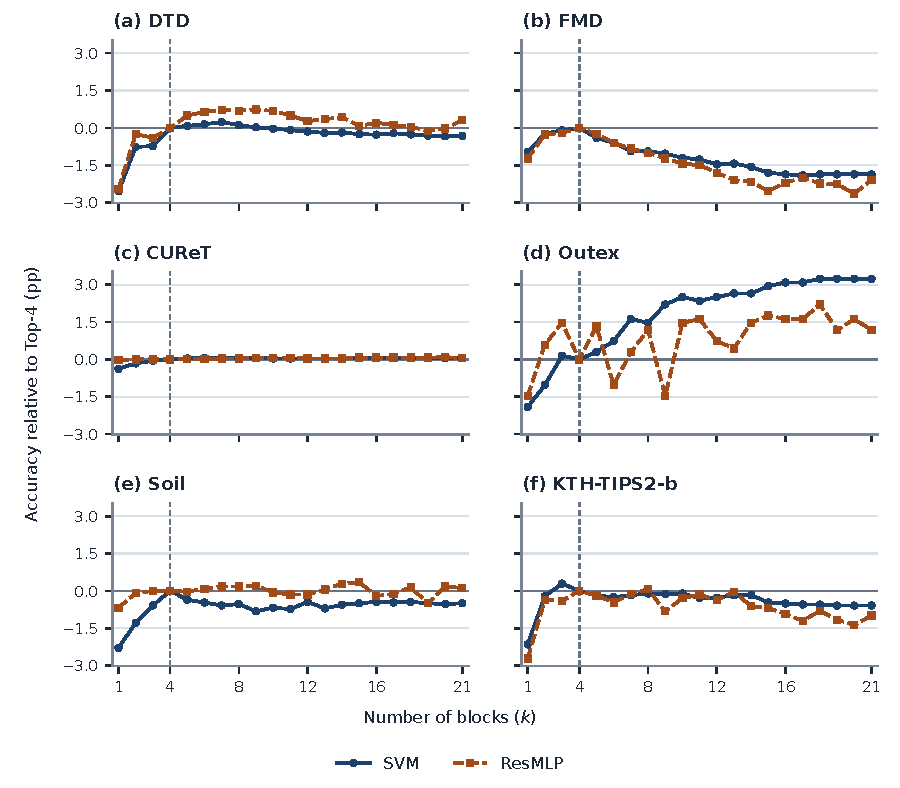
\includegraphics[width=\textwidth]{figures/english/curves_by_dataset.pdf}
\caption{Outer-test accuracy relative to direct Top-4 for each dataset and head. For each curve, zero is that head's accuracy at $k=4$ on the same dataset. Values above zero favor the indicated block count. Each point averages the outer conditions for that dataset; Outex uses one official split. The six panels share the same vertical scale.}
\label{fig:curves-by-dataset}
\end{figure}
\FloatBarrier

\subsection{Choosing the block count within training}

For each outer condition, the maximum rule takes the smallest $k$ with maximum inner macro-F1. The gain rule stops at the first $k$ for which adding block $k+1$ changes inner macro-F1 by less than the tolerance; if it never stops, it retains all 21 ranked blocks. Table~\ref{tab:k-rules} reports external accuracy using the selected size for each condition. With SVM, the maximum rule chooses 6.32 blocks on average and obtains 94.14\% accuracy, against 94.42\% at four. With ResMLP, it selects 7.26 blocks and obtains 94.30\%, against 94.20\% at four. The fixed settings and the gain rules describe smaller operating points. The choice of four blocks trades accuracy against size and depends on the head.

\begin{table}[pos=htbp]
\centering
\caption{Block-count rules applied to the inner macro-F1 curve. Entries give mean selected $k$ and outer accuracy (\%) by head. Conditions are averaged within dataset; the six datasets have equal weight.}
\label{tab:k-rules}
\small
\begin{tabular}{@{}lrrrr@{}}
\toprule
Selection rule & SVM $k$ & SVM acc. & ResMLP $k$ & ResMLP acc. \\
\midrule
Maximize inner macro-F1 & 6.32 & 94.14 & 7.26 & 94.30 \\
First gain below 0.001 & 3.23 & 94.11 & 2.15 & 93.93 \\
First gain below 0.005 & 1.92 & 93.82 & 1.71 & 93.78 \\
First gain below 0.010 & 1.68 & 93.52 & 1.30 & 93.22 \\
Fixed $k=3$ & 3.00 & 94.25 & 3.00 & 94.28 \\
Fixed $k=4$ & 4.00 & 94.42 & 4.00 & 94.20 \\
Fixed $k=6$ & 6.00 & 94.36 & 6.00 & 93.98 \\
\bottomrule
\end{tabular}
\end{table}

\subsection{Variation across archived conditions}

The pooled error counts in E1 give more weight to datasets with more test calls. DTD contributes ten conditions and 18,800 predictions in total; Outex contributes one condition and 680 predictions. In contrast, the main estimate gives the two datasets equal weight. Table~\ref{tab:e1-ranges} describes the variation observed within each dataset. Outex contributes a single change. Reused test images across splits limit the independence of these observations.

\begin{table}[pos=htbp]
\centering
\caption{Observed changes in E1. Changes are cascade minus direct accuracy, in percentage points. Gains, ties, and losses count conditions. The extrema describe the archived conditions.}
\label{tab:e1-ranges}
\small
\begin{tabular}{@{}lrrrrrrr@{}}
\toprule
Dataset & Conditions & Mean & Minimum & Maximum & Gains & Ties & Losses \\
\midrule
DTD & 10 & +0.085 & -0.319 & +0.479 & 6 & 0 & 4 \\
FMD & 5 & +0.100 & +0.000 & +0.500 & 1 & 4 & 0 \\
CUReT & 2 & -0.071 & -0.143 & +0.000 & 0 & 1 & 1 \\
Outex & 1 & -0.294 & -0.294 & -0.294 & 0 & 0 & 1 \\
Soil & 5 & +0.175 & +0.000 & +0.439 & 2 & 3 & 0 \\
KTH-TIPS2-b & 4 & +0.084 & -0.084 & +0.421 & 1 & 2 & 1 \\
\bottomrule
\end{tabular}
\end{table}

\subsection{Coverage and selected first-stage descriptors}

The E1 route is chosen separately in each outer training split, and every condition selects a cascade. SigLIP-B is the first stage in all 20 DTD, FMD, and Soil conditions. BEiTv2-B is selected in all five KTH-TIPS2-b and Outex conditions. The two complementary CUReT splits use different first stages. The selected descriptor determines both the scores used by the gate and the extractions left to perform if it escalates.

\begin{table}[pos=htbp]
\centering
\caption{Split coverage and first-stage selections with SVM. Static and E1 count outer conditions. The remaining columns count E1 conditions selecting each first-stage descriptor. E4 refits with ResMLP on the E1 splits.}
\label{tab:e1-routes}
\small
\begin{tabular}{@{}lrrrrrr@{}}
\toprule
Dataset & Static & E1 & ResNet-50 & SigLIP-B & BEiTv2-B & ConvNeXt V2-T \\
\midrule
DTD & 10 & 10 & 0 & 10 & 0 & 0 \\
FMD & 15 & 5 & 0 & 5 & 0 & 0 \\
CUReT & 2 & 2 & 1 & 0 & 1 & 0 \\
Outex & 1 & 1 & 0 & 0 & 1 & 0 \\
Soil & 15 & 5 & 0 & 5 & 0 & 0 \\
KTH-TIPS2-b & 4 & 4 & 0 & 0 & 4 & 0 \\
\bottomrule
\end{tabular}
\end{table}

\FloatBarrier

\section{Data and code availability}

The \href{https://github.com/Joafp/concatenacion-descriptores-texturas}{project repository} contains the code and evaluation records. Datasets are available from their distributors under the respective collection terms. The static curves and online metrics are consolidated in \nolinkurl{results/analysis/thesis_accuracy_primary_20261115_v3/}. Figure~\ref{fig:curves-by-dataset} uses \nolinkurl{per_dataset_curves.csv} from that directory. The online timing harness is \nolinkurl{scripts/benchmark_local_single_image.py}; the aliased runner uses the same timing boundary. Canonical coverage and timing reservations are recorded in \nolinkurl{results/analysis/blocker_resolution_20261101/full_panel_online_v1/coverage.json}. The audit of E1 and E2 is in \nolinkurl{results/analysis/top4_fixed_kth_completion_audit_20261115_v1/}. The per-image analysis and the recipe for reconstructing its counts are in \nolinkurl{carlos/analisis_paper/}. That directory contains \nolinkurl{reglas_k.awk} and \nolinkurl{reglas_k.txt}, which reproduce Table~\ref{tab:k-rules} from the archived sweeps. Table~\ref{tab:e1-ranges} comes from \nolinkurl{e1_dataset_observed_ranges.csv} in the archived sensitivity analysis \nolinkurl{results/analysis/ars_revision_existing_analyses_20261115_v1/}. Table~\ref{tab:e1-routes} tallies the \texttt{cheap} field of \nolinkurl{e1_conditions.csv}. The E4 and E5 audits are in \nolinkurl{results/analysis/e4_resmlp_complete_audit_20261116_v1/} and \nolinkurl{results/analysis/e5_top4_plus_ngram_audit_20261116_v1/}. The published figures and protocols are documented in \nolinkurl{docs/fsc_tex/METRICAS_PUBLICADAS_Y_COMPARABILIDAD_2026-11-23.md}.

\section*{Declarations}

The study uses public image collections and did not recruit participants. Funding and competing interests are pending author confirmation.

\section*{Generative AI assistance in manuscript preparation}

OpenAI Codex (GPT-6) assisted with manuscript organization, clarity, translation, LaTeX preparation, and checking manuscript counts against archived results. The authors should review this version and confirm the scope of the declaration before submission.

\bibliographystyle{unsrtnat}
\bibliography{references}
\end{document}
